\textit{Cette phase d'analyse est un élément indispensable à la bonne réalisation du projet. Dans un premier temps, un modèle plus fidèle à la réalité des schémas stockés dans les SGBDR est présenté. Cette partie est suivit d'une petite réflexion sur l'utilisation des ORM. Sont ensuite parcourus les solutions de génération de graphes pour la représentation des données. Les choic concernant l'interface utilisateur seront également exposés.}

\section{Le modèle}
\subsection{Modèle réellement rencontré}

Lors de l'étude des métadonnées stockées par les différents SGBD, nous avons remarqué quelque divergences par rapport au modèle fournit avec le sujet (figure~\ref{figure:diag_classe_fournit} page~\pageref{figure:diag_classe_fournit}). La figure~\ref{figure:diag_classe_reel} présente un diagramme de classe construit suite à nos recherches.

\begin{figure}[H]
\centering
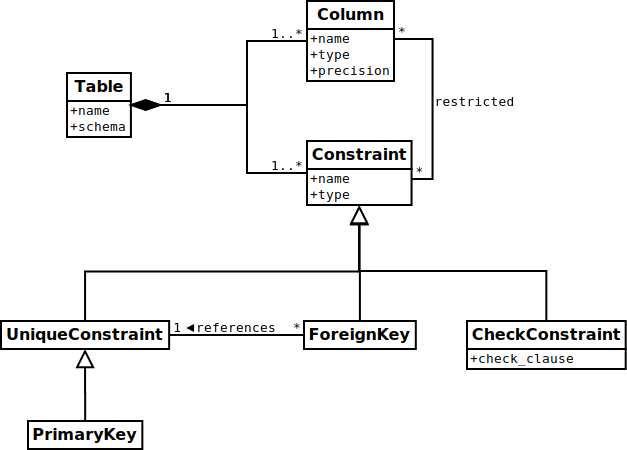
\includegraphics[width=\textwidth]{files/diag_class_ameliore}
\caption{Diagramme de classe réellement rencontré.}
\label{figure:diag_classe_reel}
\end{figure}

La principale différence réside dans la classification des contraintes. Cette classification permet de distinguer trois types de contraintes :

\begin{itemize}
\item Les contraintes d'unicité : elles contraignent l'unicité d'un ou plusieurs attributs au sein d'une même table. Les contraintes de clé primaire sont des contraintes d'unicité.
\item Les contraintes d'intégrité référentielle : elles identifient un ou plusieurs attributs d'une table comme référençant un ou plusieurs attributs d'une autre table, au travers d'une contrainte d'unicité. Notons que ce type de contrainte permet de \textbf{référencer une contrainte d'unicité et non plus une contrainte de clé primaire} comme proposé dans le modèle original.
\item Les contraintes de type \emph{Check} : qui s'appliquent à un ou plusieurs attributs d'une table. Elles contiennent une clause de vérification \texttt{check\_clause}.
\end{itemize}

\paragraph*{NB}
Les contraintes de type \emph{NULL}, \emph{NOT NULL} et \emph{DEFAULT} sont ignorées.

	\subsection{Attributs}
		Gestion des types génériques
	\subsection{Tables}
	\subsection{Contraintes}
	
\section{ORM}
\subsection{Qu'est-ce qu'un ORM ?}
\subsection{Pourquoi ?}

\section{Compatibilité avec les SGBD}

\section{Générateur de graphes}
  \subsection{différentes librairies}
		\paragraph{jung}
				entrée : un fichier dot\\
				inconvénients : dernières fonctionnalités dot non prise en charqe.
		\paragraph{grappa}
				 entrée : fichier dot
		\paragraph{graphviz}
			GraphViz est un ensemble de logiciel libre développé par AT\&T pour la visualisation de graphes. Il introduit le langage de description de graphe DOT.
				
  \subsection{Notre choix}
		\verb+//Notre choix c'est porté sur la commande DOT fournit par GraphViz+

\section{L'IHM}	
	\subsection{les choix possibles}
	\label{ihm_choix_possibles}
		Concernant la conception de l'interface utilisateur, deux choix principaux s'offrent à nous. Le premier est de concevoir
une interface graphique proposant une fenêtre de configuration puis un affichage du résultat obtenu. Le second est de concevoir 	une interface en ligne de commande générant une image. 	
	
		\subsubsection{GUI : \og Graphical User Interface \fg{}}
			Une interface utilisateur graphique permet une prise en main rapide et intuitive d'un logiciel mais ne permet pas une grande interopérabilité. En effet, il est compliqué de demandé à un programme de configurer un autre programme via une interface graphique.
			
		\subsubsection{CLI : \og Command Line Interface \fg{}}
			La conception d'une interface en ligne de commande entre dans la philosophie KISS, « Keep it simple, Stupid! ». Cette philosophie préconise la recherche de simplicité dans la conception et insiste sur le fait que toute complexité non nécessaire devrait être évitée. Cette vision à l'avantage d'offrir une grande interopérabilité, il est en effet aisé d'exécuter une ligne de commande depuis un logiciel et d'en récupérer la sortie. Par contre, une interface en ligne de commande est plus difficile à prendre en main pour un utilisateur non averti.  
			
	\subsection{Notre choix}
		Nous avons choisi pour notre logiciel, d'implémenter une interface en ligne de commande pour les avantages de cette vision, détaillés précédement en \ref{ihm_choix_possibles}, à savoir sa simplicité et sa grande interopérabilité. De plus, nous pouvons, à partir d'une interface en ligne de commande, créer une interface graphique dans un langage quelconque qui encapsule notre logiciel, alors que l'inverse est bien entendu beaucoup moins évident.

